
\documentclass[conference]{IEEEtran}
\IEEEoverridecommandlockouts

\usepackage{cite}
\usepackage{amsmath,amssymb,amsfonts}
\usepackage{graphicx}
\usepackage{textcomp}
\usepackage{xcolor}
\usepackage{hyperref}
\usepackage{etoolbox}
\usepackage[utf8]{inputenc}

\def\BibTeX{{\rm B\kern-.05em{\sc i\kern-.025em b}\kern-.08em
    T\kern-.1667em\lower.7ex\hbox{E}\kern-.125emX}} 

\begin{document}

\title{\textbf{Assignment 2: The Raven Test \\ \LARGE{In Search for Group Differences}}\\
\vspace{10pt}
\Large Data Mining, University of Aveiro \\ 2019
}

\author{\IEEEauthorblockN{Filipe Pires, 85122}
\IEEEauthorblockA{\textit{DETI, MSc. Informatics Engineering}}
\and
\IEEEauthorblockN{João Alegria, 85048}
\IEEEauthorblockA{\textit{DETI, MSc. Informatics Engineering}}

}

\makeatletter
\patchcmd{\@maketitle}
{\addvspace{0.5\baselineskip}\egroup}
{\addvspace{-1\baselineskip}\egroup}
{}
{}
\makeatother

\maketitle

\begin{abstract}
...
\end{abstract} 

\begin{IEEEkeywords}
...
\end{IEEEkeywords}

\section{Introduction}

Lorem ipsum ...

\section{Dataset \& Feature Extraction}

Lorem ipsum ...

\section{Data Quality \& Normalization}\label{data}
In relation to the dataset and the quality of the information present on it, through analysis of Table \ref{fig:feature}, which is the visual representation of the correlation of every possible pair of features, being the diagonal the pair composed of the feature with itself and is represented with a histogram that describe the value distribution inside that given feature, the remaining pairs are represented with scatter plots, we can take some important conclusions. The first one, which was already expected is that there was some outliers that needed to be taken care of, the second conclusion that's more important for this study is the fact that the data in all pairs of features doesn't appear to be separable, i.e., since there is two classes, the \textit{DEI} class and the \textit{ESEC} class there should be something resembling two groups, one for each class. That doesn't happen since in most cases we are presented with a uniform distributions, gaussian distributions or simply the grouping of all data in a unique central point. 

After familiarizing better with the data and understanding it better, it was needed to process it in a way that the models that we intend to apply have the best change of finding the distinguishing factors. For that we needed to remove the already mentioned outliers and normalize the data. We started by doing the mentioned normalization, which consisted in applying the \textit{ZSCORE} algorithm to each feature, which follows the Formula \ref{zscore} and already centers the data. Following this we also removed any data entry that contained a \textit{Null} values, since that would cause problems to the models' processing. Finally we removed the still existing outliers applying the Expression \ref{outliers}.

\begin{equation}\label{zscore}
    z_{i} = \frac{x_{i} - \mu}{\delta}
\end{equation}

\begin{equation}\label{outliers}
    |x_{i}-\mu| < 3\times\delta
\end{equation}

\section{Classifiers}\label{classifiers}
In this section we will present and give a brief summary of all the machine learning models used in this study. We chose this models since through a brief state of the art analysis we concluded that these are the most common and suggested models when handling machine learning problems, and also the ones that achieve the best performance overall. We also found that some of the models used are to most recommended when handling with data similar to our context.

\subsection{Support Vector Machine}
\textit{Support Vector Machine}, commonly denoted as SVM, is a supervised machine learning model that with the supplied training set, maps the different data entries into a multidimensional space in a way that the widest possible gap exists between the data of each class. Based in that gap a model is created and a decision rule defined that when feed new data tries to assign a class to that entry by comparing against the decision rule already mentioned.

The most common and simple SVM application tries to creates a linear division between the presented classes. Another alternative that allows more complex decision rules is the application of a kernel trick, that implicitly maps tha data to a higher-dimensioned feature space which may enable a better separation of the data.

\subsection{MultiLayer Perceptron}
\textit{MultiLayer Perceptron} is a class of feedforward artificial neural network is another supervised machine learning model. MLP is sometimes strictly refers to networks composed of multiple layers of perceptrons. Perceptron is also a supervised learning algorithm capable of doing binary classifications according to a linear predictor function. The power of the MLP is the junction of several of those perceptrons that individually don't have the a good performance, but the combine performance can reach significant values.

This junction normally follows a standard architecture divided in layers, firstly a input layer, followed by one or more hidden layers and an output layer. The input and the output layers are the ones that interact with the exterior, being the first, as the name indicates teh one where the data should be injected at and the second where the result will be presented. The hidden layers is where the main learning occurs and where the most amount of fine-tunning is applied. In this entire architecture the number of layers and the number of neurons(singular cell inside a layer) can be tunning to improve the model performance.

\subsection{Decision Tree}
This supervised learning algorithm, as the name suggests, uses a tree like structure to support the data classification decision and aims to convert the observed patterns in the train data into conclusions about the data classes. The construction of this auxiliary structure is quite simple and straightforward, consisting in assigning a condition to each new branch, causing that the structure will converge in having only one class in leaf nodes, defining the conditions required to identify the existing classes. These condition choices must be taken with caution since a poor decision in this phase may cause a drastic decrease in the performance of the overall model. Many times this process uses \textit{Entropy} as a guide, where \textit{Entropy} indicates, in a very high level approximation, the level of confusion/chaos/randomness of a set of information, thereby if the data tested belongs to only one class, the entropy should be 0 and the system knows that that data portion doesn't need to be divided anymore.

\subsection{Random Forest}
Similarly to the last model, \textit{Random Forest} is also a supervised learning model and also uses tree structures to support the models' classification decisions. The difference is that in this approach the model uses several instances of Decision Trees, with the purpose of since sometimes Decision Tree don't generate the best performance possible, using multiple and dividing the problem so that not every tree specializes in all the features, dividing and conquering the problem.

\subsection{K Nearest Neighbors}
The last model that we decided to test was the \textit{K Nearest Neighbors}, which although being one of the simplest learning algorithms, still is essential in the Machine Learning area. Still in the supervised learning algorithm area, this model uses a very simple approach to it's classification process; by representing every train data entry in a multidimensional space, once presented with new data, the model simple represents that new entry in the mentioned multidimensional space and verifies the class of the K nearest points(train entries), and the most frequent class in that K dataset is the one that is assigned to that new data entry. 

\section{Parameters Variation}\label{parameters}

Lorem ipsum ...

\section{Results Discussion}
After executing all the parameter variation study, the feature analysis as well as some feature addition in hopes of adding some extra meaningful information to the already existing data, the best performance results were the ones presented in Section \ref{parameters}.
Although not the most satisfying results, since when conducting a machine learning problem the aim is to obtain a model with a defined set of hyperparameters that generate a good performance with good values(close to 100\%) on its performance indicators, but the results obtained in this study have a reason to be.

Referring to Section \ref{data}, one of the conclusions taken from analyzing the Figure \ref{fig:feature} was that no obvious division was observable in the data projections in the different feature pair plane. Although this conclusion not absolute proof that the data isn't separable, the results of the tested model indicate that that is the case. This can be caused by several reasons, ranging from the dataset quality, the models used, the tunning of the hyperparameters or even the case of overfitting of the training data. 

Through a deeper analysis over the data itself we didn't found any aspect that could compromise our study; the origin of the data and the metrics gathered seemed to be the most adequate for this type of study; the features also seemed to be widespread enough to encapsule all the possible signals related to this study, such as fatigue, immersion, stress, \dots. In relation to the models used, as already mentioned in Section \ref{classifiers} are state-of-the-art, therefor should perform well enough with the dataset presented, and for that matter, with any dataset. The parameters variation was probably the portion of the report study that took the longer, since we made a meticulous study of the parameters for all the models trained as detailed in Section \ref{parameters}. For that reason we can conclude that the parameter choice is also not the problem. Finally, in relation to the overfitting problem, the fact that all the models used gave similar results, it's quite improbable that all of them suffer from the overfitting. That allows us to also remove this problem from our list of possible issues.

Knowing that the variables in our reach are properly tested and in theory are correct, we can only conclude that the data itself is inseparable. This means that the two classes presented, the students from \textit{DEI} and the students from \textit{ESEC}, although obviously two different groups in this study, the conducted experiment indicates that in terms of the \textit{RAVEN} intelligence estimation test there is no difference between the two groups.

Finally, in spite of all models produced a similar performance, where the \textit{Accuracy} averaged in the 55\% mark and the \textit{F-Score} averaged in the 65\% mark. This difference is due to the fact that both \textit{Precision} and \textit{Recall} are slightly higher than the \textit{Accuracy}, which indicates that however the classification is almost random, in reality the models are able to generate more true results than negative results, which is quite interesting given the limitations observed from the models.

\section{Conclusions \& Future Work}
In conclusion, we verify that the two groups can be distinguished through their intelligence. This conclusion was expected since belonging to different backgrounds doesn't automatically imply that a person is smarter or not, simply as a different area of interest.

% \begin{itemize}
% \item Lorem ipsum ...
% \end{itemize}

% \begin{equation}
% a+b=\gamma\label{eq}
% \end{equation}

% ... \eqref{eq} ...

% ... Fig.~\ref{fig} ...

% \begin{table}[htbp]
% \caption{Table Type Styles}
% \begin{center}
% \begin{tabular}{|c|c|c|c|}
% \hline
% \textbf{Table}&\multicolumn{3}{|c|}{\textbf{Table Column Head}} \\
% \cline{2-4} 
% \textbf{Head} & \textbf{\textit{Table column subhead}}& \textbf{\textit{Subhead}}& \textbf{\textit{Subhead}} \\
% \hline
% copy& More table copy$^{\mathrm{a}}$& &  \\
% \hline
% \multicolumn{4}{l}{$^{\mathrm{a}}$Sample of a Table footnote.}
% \end{tabular}
% \label{tab1}
% \end{center}
% \end{table}

% \begin{figure}[h!]
% \centering
% \includegraphics[width=0.95\linewidth]{../img/screenshots/screenshot_map.png}
% \caption{Screen capture of our prototype's world map.}
% \label{fig:worldmap}
% \end{figure}

% \begin{figure}[htbp]
% \centerline{\includegraphics{fig1.png}}
% \caption{Example of a figure caption.}
% \label{fig}
% \end{figure}

\begin{thebibliography}{00}
\bibitem{assign2} A. Tomé, "Data Mining Assignment", \url{https://elearning.ua.pt/pluginfile.php/1496406/mod_resource/content/3/ED_HCT_Raven.pdf}, accessed in November 2019.
\end{thebibliography}
% https://en.wikipedia.org/wiki/Support-vector_machine
% https://en.wikipedia.org/wiki/Multilayer_perceptron
% https://en.wikipedia.org/wiki/Perceptron
% https://en.wikipedia.org/wiki/Decision_tree
% https://en.wikipedia.org/wiki/K-nearest_neighbors_algorithm
\vspace{12pt}

\clearpage
\appendix
\begin{figure}[h]
    \centering
    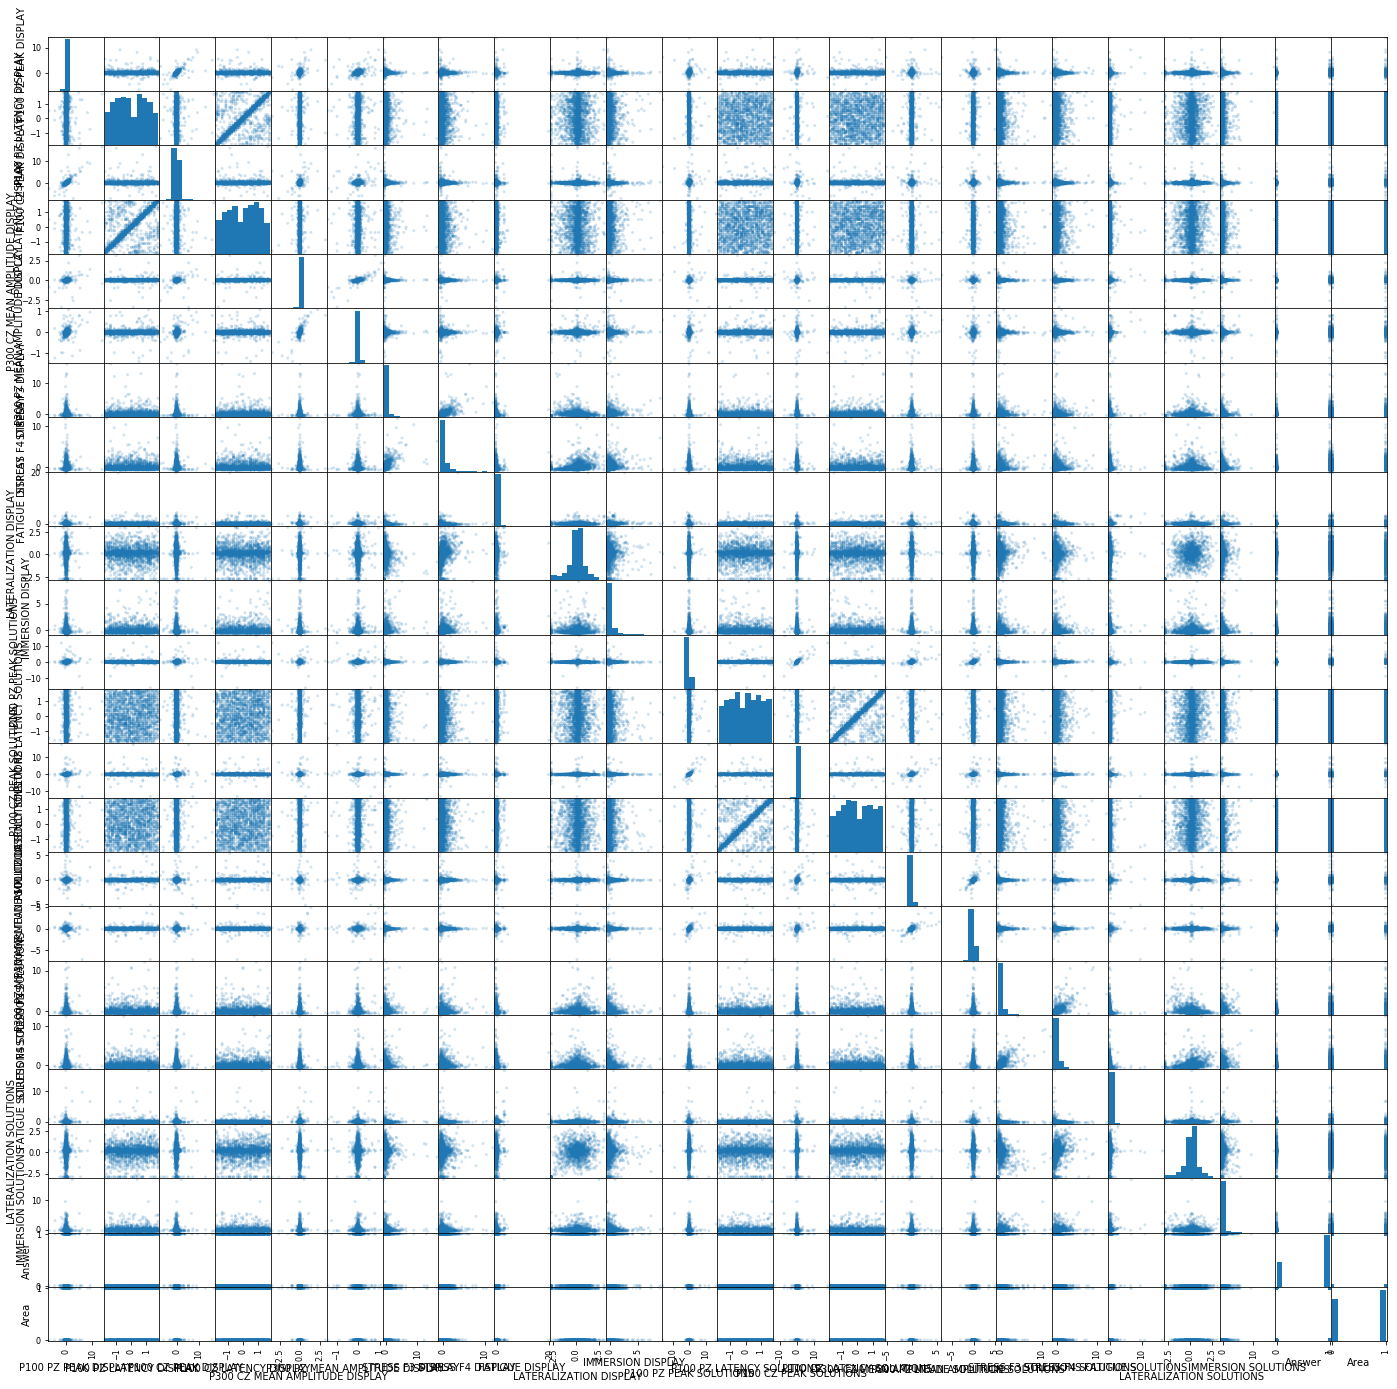
\includegraphics[width=2\linewidth]{featurecorrelation.png}
    \caption{Feature Correlations}
    \label{fig:feature}
\end{figure}

\end{document}
